\section{Cahier des charges}
    \label{sec:cahier}

    Comme indiqué dans la Section \ref{sec:objectifs}, notre principal objectif est de réaliser un logiciel aidant à l'analyse de la sécurité d'un système\footnote{La nature du dit système peut être très vaste, allant d'un simple distributeur de billets au réseau de transport de toute une ville.}. Destiné aux experts en sécurité des entreprises, notre logiciel utilisera le concept d'ADTrees décrit dans la Section \ref{sec:etat_art}. Il sera développé pour la plate-forme Microsoft Windows.

    Nous repartirons sur la base d'ADTool pour réaliser notre logiciel, afin de ne pas réécrire l'existant. Toutefois, diverses fonctionnalités que nous avons jugé utiles seront développées :
    \begin{itemize}
        \item trouver le chemin d'attaque optimal selon une fonction de synthèse, qui utilisera plusieurs paramètres (Section \ref{sec:fct_synth}).
        \item filtrer l'arbre en fonction d'une fourchette de critères (Section \ref{sec:filtre}).
        \item utiliser des modèles d'arbres généraux que l'utilisateur pourra ensuite modifier en fonction de sa situation (Section \ref{sec:modele}).
        \item améliorer l'édition des arbres avec ADTool, afin de la rendre plus souple et plus pratique (Section \ref{sec:adtoolpp}).
        \item créer un guide afin de proposer à l'utilisateur une méthode d'analyse (Section \ref{sec:guide}).
    \end{itemize}

    Pour finir, nous décrirons l'architecture de notre logiciel dans la Section \ref{sec:archi}.

    \subsection{Fonction de synthèse et chemin optimal}
        \label{sec:fct_synth}

        Dans la version actuelle d'ADTool, il est possible d'utiliser un seul paramètre à la fois sur un arbre. Pourtant, pouvoir faire une synthèse à partir de différents paramètres peut permettre de rechercher des compromis plus facilement.
        Par exemple, si on souhaite rechercher l'attaque la moins coûteuse financièrement, sans pour autant sacrifier le temps passé à réaliser notre attaque, on pourrait fournir une fonction définie par \[ synthese(cout, tps) = 2*cout + tps . \]
        Avec cette fonction, une nouvelle valuation de l'arbre sera calculée et on pourra ensuite l'élaguer pour garder uniquement les branches permettant de minimiser la fonction de synthèse.
        L'arbre élagué sera ensuite affiché, et l'utilisateur pourra prendre la décision de l'enregistrer comme un nouvel arbre.

        Afin d'obtenir le plus grand choix de fonctions possibles, nous donnerons à l'utilisateur la possibilité de combiner les différents paramètres de façon linéaire, polynomiale, et aussi d'utiliser des fonctions mathématiques \og standards \fg, comme l'exponentielle, le logarithme, etc.

    \subsection{Filtre à critères}
        \label{sec:filtre}

        Une autre fonctionnalité que nous développerons sera le filtre à critères. Les critères consistent en un ensemble de valeurs autorisées pour nos paramètres, et seront gardés uniquement les nœuds respectant ces règles. Ceci permettra d'obtenir rapidement les attaques réalisables en fonction des ressources de l'attaquant, nous permettant de modéliser plusieurs attaquants théoriques\footnote{Un étudiant et un syndicat du crime organisé n'auront pas les mêmes moyens financiers par exemple.}.
        
        Supposons qu'il existe trois sous-arbres A, B et C pour atteindre un objectif, avec un coût respectivement de 2596 €, 70333 € et 200 €. Le temps passé à réaliser l'attaque dure 1, 2 et 3 semaines. On voudrait garder uniquement les attaques qui coûtent moins de 30000 €, et qui prennent moins d'une semaine. Notre filtre supprimera donc les sous-arbres B et C, pour garder uniquement le A.

        L'arbre obtenu à l'issue du filtrage pourra très bien être identique à celui fourni en entrée (toutes les attaques respectent les critères), ou au contraire être vide (aucune attaque n'est réalisable avec les moyens alloués). Ce nouvel arbre sera ensuite affiché à l'utilisateur, qui pourra décider de l'enregistrer comme un nouvel arbre.

    \subsection{Modèles généraux}
        \label{sec:modele}

        Commencer une nouvelle étude peut parfois être difficile. Pouvoir se baser sur des études déjà réalisées pour les adapter à sa situation simplifie grandement la tâche. Ainsi, nous donnerons à l'utilisateur la possibilité de partir de modèles d'attaques existantes, qu'il devra ensuite éditer pour que l'arbre corresponde à son système. Dans notre cas d'étude, nous pourrions imaginer avoir un modèle générique d'attaque de réseau de transport en commun, pour ensuite l'éditer afin de prendre en compte les spécificités de l'agglomération rennaise et du STAR.

        Notre logiciel intégrera divers arbres génériques, mais l'utilisateur pourra aussi en importer depuis d'autres sources (Internet, clé usb, etc.). Notre logiciel étoffera sa collection de modèles à chaque nouveau modèle importé par l'utilisateur.
        L'utilisateur sera aussi capable de créer ses propres modèles, pour s'en resservir dans d'autres de ses analyses, ou encore pour les publier sur Internet. Ainsi, on pourrait imaginer à terme un site web regroupant des milliers de modèles réalisés par un réseau d'experts en sécurité.

    \subsection{Amélioration d'ADTool}
        \label{sec:adtoolpp}

        Bien qu'ADTool soit déjà très complet, nous avons identifié plusieurs fonctionnalités qui rendraient la manipulation des arbres plus aisée :
        \begin{itemize}
            \item Une fonction de couper / copier / coller d'arbres et de sous-arbres.
            \item Réaliser des glisser / déposer d'arbres et de sous-arbres.
            \item Importer et exporter des arbres dans un grand nombre de formats différents.
            \item Permettre la représentation d'un arbre avec plusieurs paramètre à la fois.
        \end{itemize}

    \subsection{Guide}
        \label{sec:guide}

        L'utilisateur n'étant pas nécessairement familier avec les ADTrees, le guide lui permettra de comprendre rapidement comment réaliser ses arbres, et comment réaliser son analyse.

        Notre guide lui fera suivre une méthode générique~\cite{methode_analyse}, découpée en différentes étapes. Une fois que l'une d'entre elles sera complétée, le guide passera à l'étape suivante et expliquera précisément à l'utilisateur comment la réaliser.
        Le guide prendra la forme d'un \og journal de quête \fg, ce qui lui permettra de garder une trace des étapes déjà réalisées.

    \subsection{Architecture}
        \label{sec:archi}

        L'architecture de notre logiciel est présentée sur la Figure \ref{fig:archi}.   

        \begin{figure}
            \begin{center}
                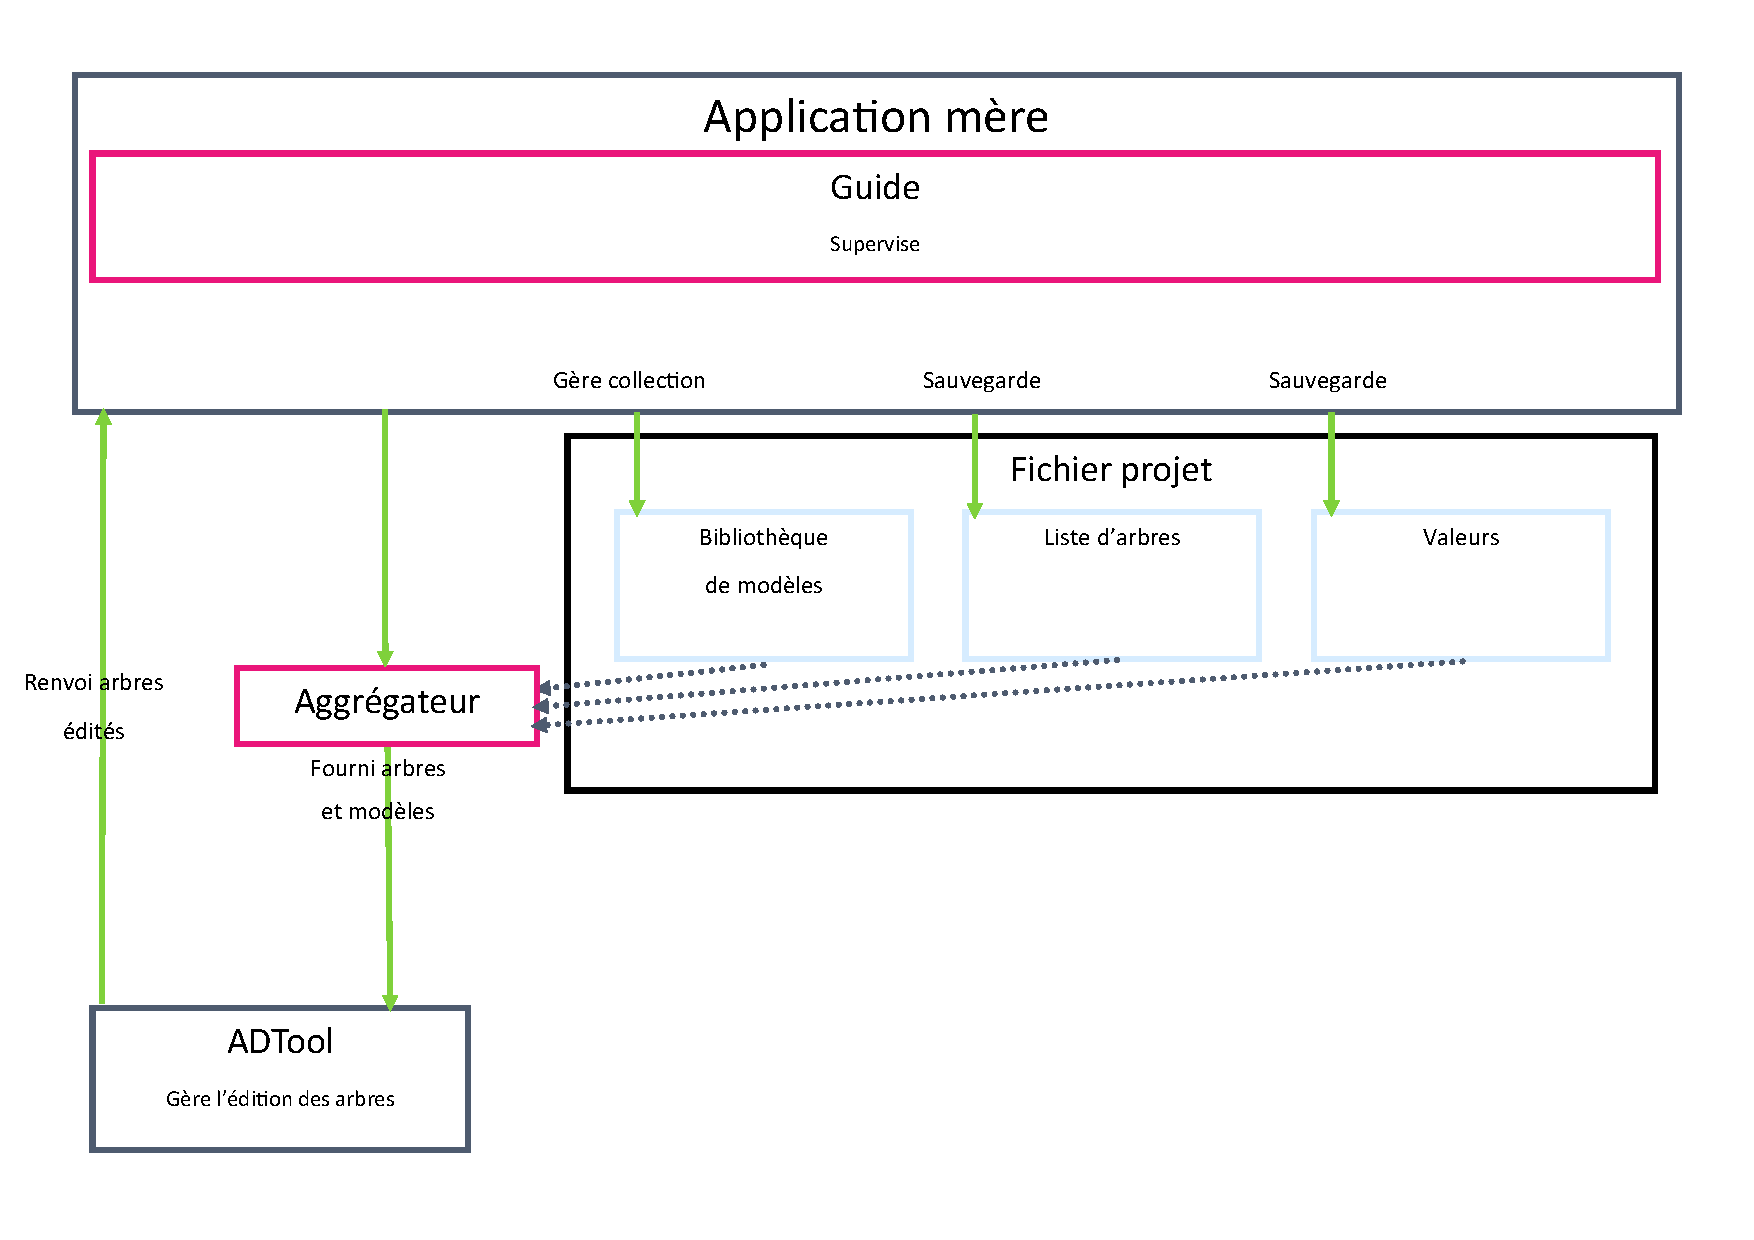
\includegraphics[width=1\textwidth]{figure/archi.pdf}
            \end{center}
            \caption{Différents modules graviteront autour d'ADTool pour atteindre nos objectifs.}
            \label{fig:archi}
        \end{figure}

        Toutes les modifications ne seront pas intégrées directement dans ADTool (seules les modifications de la Section \ref{sec:adtoolpp} y seront implémentées). \`A la place, nous auront une application mère, qui se servira d'ADTool comme étant un composant dédié à la visualisation et à l'édition des arbres. 

        L'analyse d'un système sera sauvegardée sous forme de projet. Celui-ci contiendra différents arbres utilisés pour l'analyse, ainsi qu'une bibliothèque de modèles que l'utilisateur pourra reprendre à tout moment pour créer un nouvel arbre (groupe "Fichier Projet"). 
        \`A la création du projet, une série de questions sera posée à l'utilisateur. Les réponses obtenues permettront de sélectionner un sous-ensemble des modèles de la bibliothèque du logiciel, pour les précharger dans la bibliothèque du projet.

        Les autres grandes parties de notre application (section \ref{sec:filtre}, \ref{sec:modele} et \ref{sec:guide}) seront implémentées sous forme de modules dédiés à leur tâche.
        La fonction de synthèse et le filtre seront deux modules qui prendront en entrée un arbre du fichier projet (et leurs autres paramètres respectifs), et enverront le résultat à ADTool pour affichage. L'utilisateur décidera ensuite de ce qu'il fera de l'arbre généré (sauvegarde, édition, export, etc.).
        Le guide supervisera l'ensemble de l'application, et devra fournir des informations et consignes pertinentes à l'utilisateur afin de l'aider dans son analyse.

        Une ébauche de l'interface se situe Figure \ref{fig:interface}. Notons que le guide n'y figure pas, puisqu'il ne sera pas affiché en permanence pour ne pas surcharger l'interface. Il s'agira plutôt d'une fenêtre dédiée qui pourra être ouverte et fermée au besoin.

        \begin{figure}
            \begin{center}
                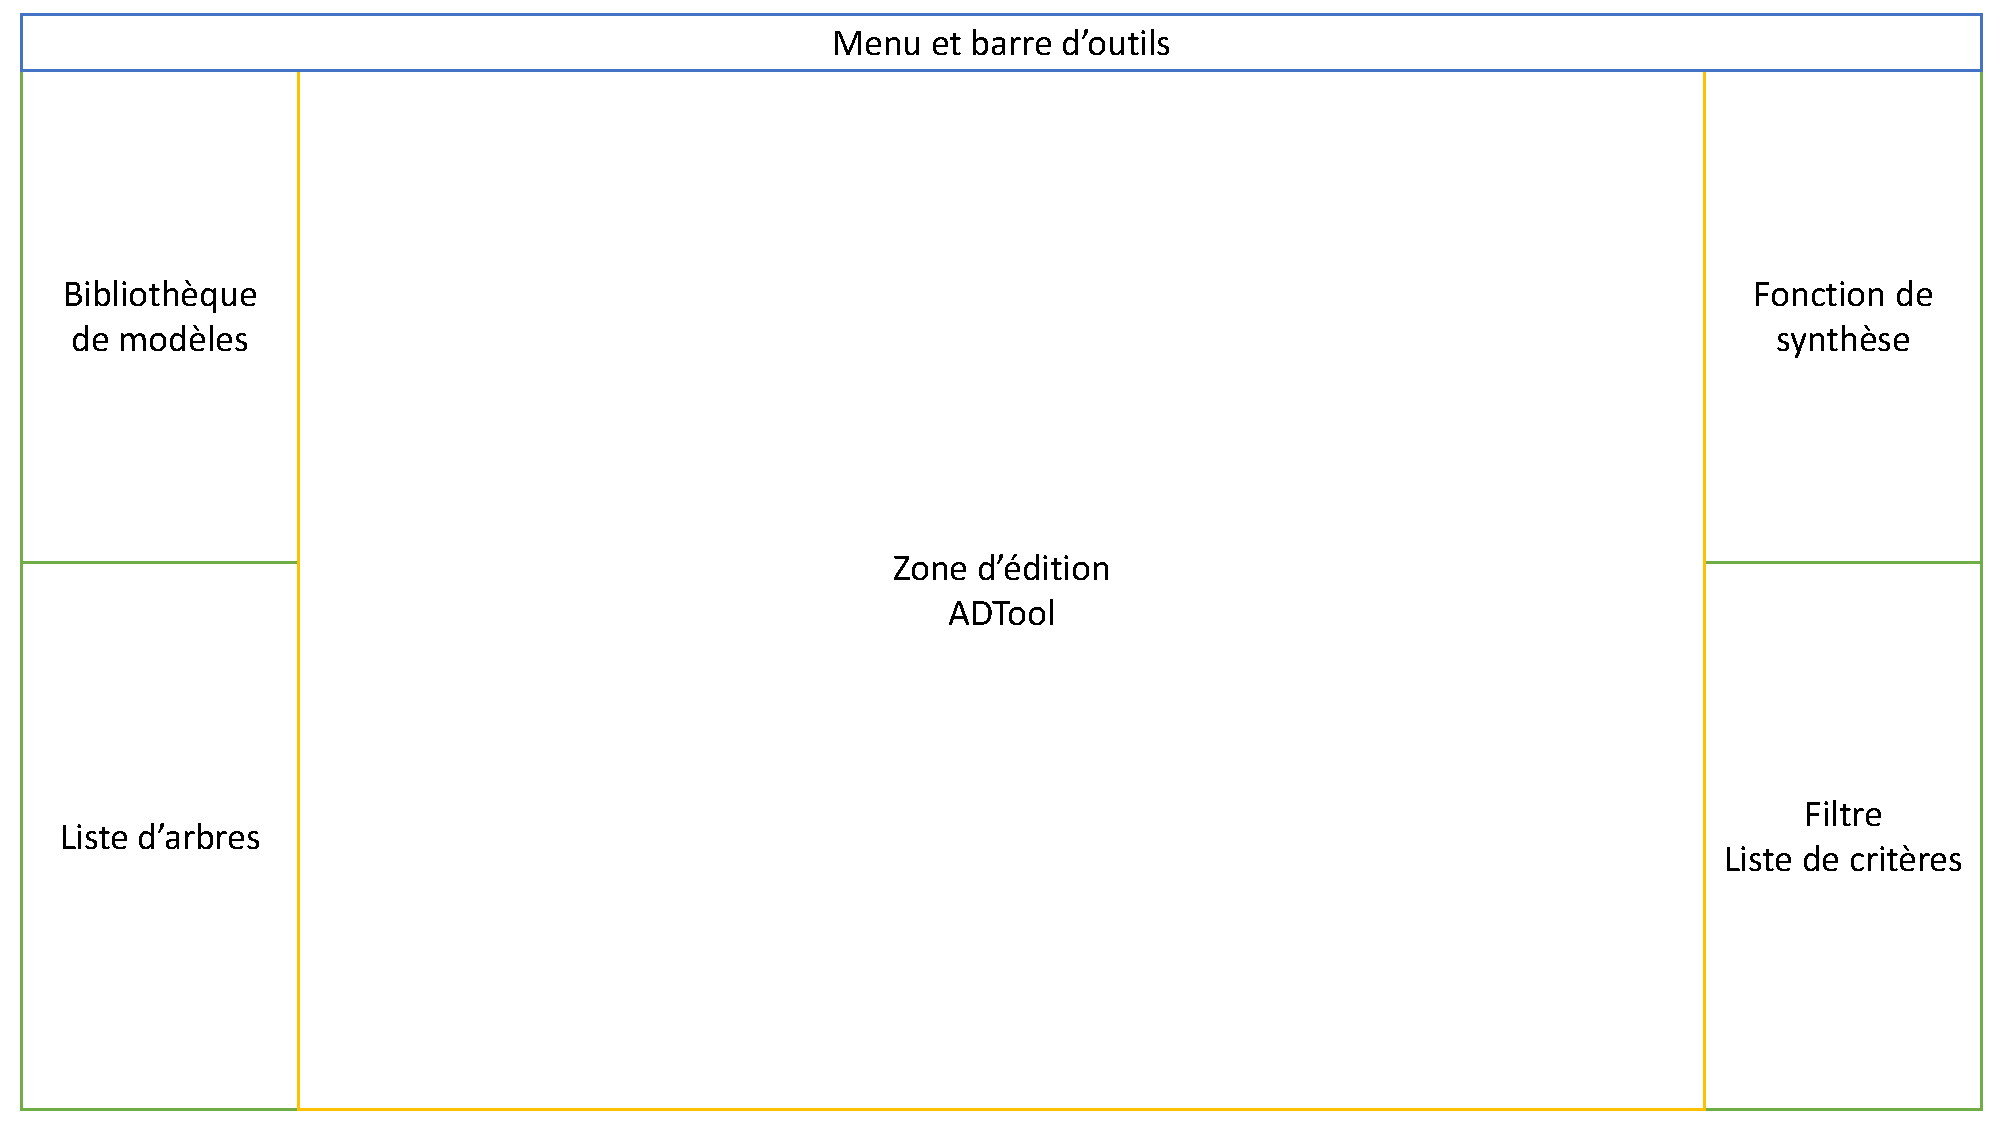
\includegraphics[width=1\textwidth]{figure/interface.pdf}
            \end{center}
            \caption{L'interface sera gardée au plus simple.}
            \label{fig:interface}
        \end{figure}